\documentclass[10pt,a4paper]{article}
\usepackage[utf8]{inputenc}
\usepackage{amsmath}
\usepackage{amsfonts}
\usepackage{amssymb}
\usepackage{listings}
\usepackage{xcolor}
\usepackage{array}
\usepackage{graphicx}
\setlength{\extrarowheight}{2pt}

\lstdefinestyle{myStyle}{
    belowcaptionskip=1\baselineskip,
    breaklines=true,
    frame=none,
    numbers=none, 
    basicstyle=\footnotesize\ttfamily,
    keywordstyle=\bfseries\color{green!40!black},
    commentstyle=\itshape\color{purple!40!black},
    identifierstyle=\color{blue},
    backgroundcolor=\color{gray!10!white},
}

\title{CS3523:OS-2 \\Programming assignment-2:Sudoku Validator}
\author{CS21BTECH11055- ABHINAY SADINENI}
\begin{document}
\maketitle
\section{Code design}
To validate sudoku we need to checks:
\begin{enumerate}
\item all rows
\item all cloumns
\item all subgrids of size $\sqrt{N}\times\sqrt{N}$ where N is size of sudoku
\end{enumerate}
it takes almost same time to validate whether it is a row,cloumn or  subgrid.it is best to distrbute them among all threads to balance the load. 
\section{Implemenation}
\begin{enumerate}
\item distribution of load same for both pthreads and openmp.
evenly divided among all threads
\begin{lstlisting}[style=myStyle]
for (int i = 1; i <=K; i++)
    {
        params*p=malloc(sizeof(params));
       if(i<=(3*N)%K){
            p->start=start;
            p->size=(3*N)/K+1;
            start=start+p->size;
       }
       else
       {
            p->start=start;
            p->size=(3*N)/K;
            start=start+p->size;
       }
        pthread_create(&tid[i-1],NULL,thread_work,(void*)p);
    }
\end{lstlisting}
\item threads work to validate its given load and store the result of each validation in the valid array
\\

   
\begin{tabular}{| *{9}{c |}}
\hline
row1 &row2 &..... &col1&col2&.....& subgrid1 & subgrid2 &.....\\
\hline
\end{tabular}
\\
$\uparrow$\\
index i inside thread work, N rows,N columns,N subgrids
\begin{lstlisting}[style=myStyle]
void  thread_work(params* p){

    for (int i = p->start; i < p->start+p->size; i++)
    {
        if(i<N){
            valid[i]=row_check(i);
        }
        else if(N<=i && i<2*N)
        {
              valid[i]=col_check(i-N);
        }
        else
        {
            valid[i]=grid_check(i-2*N);
        }
        
    }
}
\end{lstlisting}
\item function to validate a row
\begin{lstlisting}[style=myStyle]
int row_check(int j){
    bool*check=calloc(N,sizeof(bool));

    for (int i = 0; i < N; i++)
    {
        int temp=mat[j][i]-1;
      if(check[temp]==false){
        check[temp]=true;
      }
      else
      {
        free(check);
        return 0;
      }
     }
     free(check);
    return 1;
    

}
\end{lstlisting}
\item function to validate a column
\begin{lstlisting}[style=myStyle]
int col_check(int j){
    bool*check=calloc(N,sizeof(bool));
    for (int i = 0; i < N; i++)
    {
       int temp=mat[i][j]-1;
       if(check[temp]==false){
        check[temp]=true;
      }
      else
      {
        free(check);
        return 0;
      }
     }
     free(check);
    return 1;
}
\end{lstlisting}
\item function to validate a subgrid
\begin{lstlisting}[style=myStyle]
int grid_check(int j){
    int sp=sqrt((double)N);
    bool*check=calloc(N,sizeof(bool));
     for (int i = (j%sp)*sp; i <(j%sp)*sp+sp; i++)
     {
        for (int k = (j/sp)*sp; k <(j/sp)*sp+sp; k++)
        {
           int temp=mat[i][k]-1;
           if(check[temp]==false){
        check[temp]=true;
      }
      else
      {
        free(check);
        return 0;
      }
            
        }
        
     }
     free(check);
    return 1;
}
\end{lstlisting}

In all the three functions we check whether all 1 to N numbers are present or not if there is a repetition of number then function immediately returns false.

\item This below code block searches all the valid array for false 
and declares the whether the sudoku is valid or not
\begin{lstlisting}[style=myStyle]
int check=1;
    for (int i = 0; i < 3*N; i++)
    {
       if (valid[i]==0)
       {
         check=0;
         break;
       }
    }
\end{lstlisting}

\end{enumerate}
The openmp code is done in the same way except for some small changes like replacing pthread$\_$ create and pthread$\_$join with omp library syntax
\pagebreak
\section{Performance Analysis}
\subsection{Graph: Time Taken v/s N}
\begin{figure}[!ht]
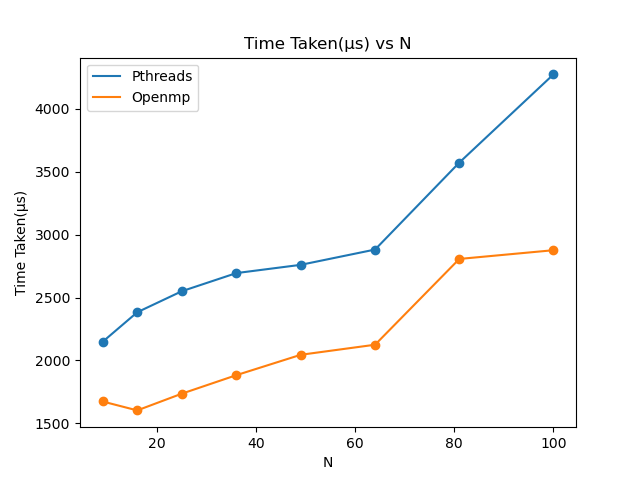
\includegraphics[scale = 0.8]{plot_const_K}
\label{Fig}
\caption{T v/s N(constant K=16)}
\end{figure}
\textbf{Observations:}
\begin{enumerate}
\item On observing carefully their is regular trend for both pthreads and openmp as the size of the sudoku the number of validations per each thread increases so therefore time taken also increases
\item There is slight defect of trend in openmp i.e. slight decrease at N=4  this maybe because of some CPU scheduling at the time of excecution.
\item Openmp's performance better than pthreads this is because openmp optimizes sequentail code blocks 
\end{enumerate}
\pagebreak
\subsection{Graph: Time Taken v/s No of threads }
\begin{figure}[!ht]
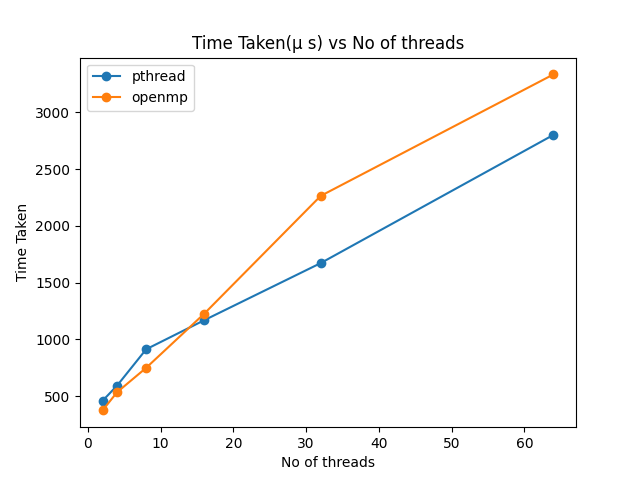
\includegraphics[scale = 0.8]{plot_final_25}
\label{}
\caption{T v/s K (N=25 constant)}
\end{figure}
\textbf{Observations:}
\begin{enumerate}
\item We expect the time taken to decrease
\item But here the value of N is just 25 ,in which case the overhead of creation of threads exceeds the speed up by threads.
\item Usually threads speedup  is significent when there is large amount of load.
\item for checking just 625 cells in a sudoku threads are not needed.
\item This given input works faster with normal iteration method.
\item CPU(intel i5-1035G1) has only 4 cores thats why at N=16 the openmp plot crosses the pthread plot.
\end{enumerate}
\subsection{Conculsion:}
\begin{enumerate}
\item Openmp implementation works better than that of pthreads
\item But we cannot conclude with that one fact, since the omp threads also depend on number of cores avialable and architecture of the chip more than pthreads as seen in second graph
\end{enumerate}
\end{document}